% !TEX program = xelatex
\documentclass[a4paper, 14pt]{report}

% Подключение необходимых пакетов для XeLaTeX
\usepackage{fontspec}                 % Для управления шрифтами
\usepackage{polyglossia}              % Для поддержки многоязычности
\setmainlanguage{russian}             % Установка основного языка
\setotherlanguage{english}            % Дополнительный язык (если требуется)
\newfontfamily\cyrillicfonttt{Courier New} % Шрифт для моноширинного текста
% Установка основного шрифта
\setmainfont{Times New Roman}

% Пакеты для оформления документа
\usepackage{geometry}                 % Параметры полей
\usepackage{setspace}                 % Межстрочный интервал
\usepackage{titlesec}                 % Настройка заголовков
\usepackage{graphicx}                 % Вставка изображений
\usepackage{caption}                  % Настройка подписей
\usepackage{subcaption}               % Подписи подрисунков
\usepackage{tocloft}                  % Настройка оглавления
\usepackage{hyperref}                 % Гиперссылки
\usepackage{listings}                 % Вставка исходного кода
\usepackage{xcolor}                   % Цвета для оформления кода
\usepackage{float}                    % Плавающие изображения
\usepackage{fontawesome5}             % Иконки
\usepackage{tcolorbox}                % Цветные блоки
% Настройка геометрии страницы
\geometry{
    a4paper,
    left=30mm,
    right=20mm,
    top=10mm,
    bottom=10mm,
    footskip=0mm
}

\bibliographystyle{gost-numeric.bbx}
\usepackage[style=numeric, backend=biber]{biblatex}
\addbibresource{ref/references.bib}

% Межстрочный интервал 1.5
\onehalfspacing

% Настройка заголовков
\titleformat{\chapter}[block]
  {\centering\bfseries\Large} % Форматирование заголовка
  {\chaptername\ \thechapter}{1em}{}

\titleformat{\section}
  {\centering\bfseries\large}
  {\thesection}{1em}{}

\titleformat{\subsection}
  {\centering\bfseries\normalsize}
  {\thesubsection}{1em}{}

% % Оглавление без точек после номеров
% \renewcommand{\cftsecleader}{\cftdotfill{\cftdotsep}}

% Подключение пакета listingsutf8 для поддержки UTF-8 в листингах
\usepackage{listingsutf8}

% Включение ссылок в оглавлении
\setcounter{tocdepth}{3}

% Настройки для листингов кода
\lstset{
    basicstyle=\ttfamily\small,
    keywordstyle=\color{blue},
    commentstyle=\color{gray},
    stringstyle=\color{red},
    numbers=left,
    numberstyle=\tiny,
    stepnumber=1,
    numbersep=5pt,
    tabsize=4,
    breaklines=true,
    breakatwhitespace=false,
    showstringspaces=false,
    frame=single
}
\makeatletter % see https://tex.stackexchange.com/a/320345
\lst@InputCatcodes
\def\lst@DefEC{%
 \lst@CCECUse \lst@ProcessLetter
  ^^80^^81^^82^^83^^84^^85^^86^^87^^88^^89^^8a^^8b^^8c^^8d^^8e^^8f%
  ^^90^^91^^92^^93^^94^^95^^96^^97^^98^^99^^9a^^9b^^9c^^9d^^9e^^9f%
  ^^a0^^a1^^a2^^a3^^a4^^a5^^a6^^a7^^a8^^a9^^aa^^ab^^ac^^ad^^ae^^af%
  ^^b0^^b1^^b2^^b3^^b4^^b5^^b6^^b7^^b8^^b9^^ba^^bb^^bc^^bd^^be^^bf%
  ^^c0^^c1^^c2^^c3^^c4^^c5^^c6^^c7^^c8^^c9^^ca^^cb^^cc^^cd^^ce^^cf%
  ^^d0^^d1^^d2^^d3^^d4^^d5^^d6^^d7^^d8^^d9^^da^^db^^dc^^dd^^de^^df%
  ^^e0^^e1^^e2^^e3^^e4^^e5^^e6^^e7^^e8^^e9^^ea^^eb^^ec^^ed^^ee^^ef%
  ^^f0^^f1^^f2^^f3^^f4^^f5^^f6^^f7^^f8^^f9^^fa^^fb^^fc^^fd^^fe^^ff%
  ^^^^20ac^^^^0153^^^^0152%
  % Basic Cyrillic alphabet coverage
  ^^^^0410^^^^0411^^^^0412^^^^0413^^^^0414^^^^0415^^^^0416^^^^0417%
  ^^^^0418^^^^0419^^^^041a^^^^041b^^^^041c^^^^041d^^^^041e^^^^041f%
  ^^^^0420^^^^0421^^^^0422^^^^0423^^^^0424^^^^0425^^^^0426^^^^0427%
  ^^^^0428^^^^0429^^^^042a^^^^042b^^^^042c^^^^042d^^^^042e^^^^042f%
  ^^^^0430^^^^0431^^^^0432^^^^0433^^^^0434^^^^0435^^^^0436^^^^0437%
  ^^^^0438^^^^0439^^^^043a^^^^043b^^^^043c^^^^043d^^^^043e^^^^043f%
  ^^^^0440^^^^0441^^^^0442^^^^0443^^^^0444^^^^0445^^^^0446^^^^0447%
  ^^^^0448^^^^0449^^^^044a^^^^044b^^^^044c^^^^044d^^^^044e^^^^044f%
  ^^^^0401^^^^0451%
  %%%
  ^^00}
\lst@RestoreCatcodes
\makeatother

\renewcommand\thesection{\arabic{section}}

\begin{document}
\newcommand{\nchapter}[1]{%
    \chapter*{#1} % Заголовок главы без нумерации
    \addcontentsline{toc}{chapter}{#1} % Добавление в оглавление
}
\newcommand{\nsubsection}[1]{%
    \subsection*{#1} % Заголовок главы без нумерации
    \addcontentsline{toc}{subsection}{#1} % Добавление в оглавление
}
\makeatletter

% Table of contents in chapter style
\renewcommand{\tableofcontents}{%
    \chapter*{\contentsname}%
    \addcontentsline{toc}{chapter}{\contentsname}%
    \@starttoc{toc}%
}
\makeatother

% Титульный лист
\begin{titlepage}
    \centering
    {\large Федеральное государственное автономное образовательное учреждение высшего образования}\\
    {\large «Национальный исследовательский университет ИТМО»}\\[0.5cm]

    {\large Факультет программной инженерии и компьютерной техники}\\[3cm]

    {\large \bfseries Вопрос-ответ}\\[0.5cm]
    {\large \bfseries «Учетные записи и авторизация в ОС MS Windows»}\\[0.5cm]
    {\large по дисциплине}\\[0.5cm]
    {\large \bfseries «Информационная безопасность»}\\[1cm]

    {\large Вариант № \underline{49}}\\[5cm]
    \begin{flushright}
        {\large \underline{Группа: P34102}}\\[0.5cm]
        {\large \underline{Выполнил:} Лапин А.А.}\\[1cm]

        {\large \underline{Проверил:}}\\
        {\large Рыбаков С.Д.}\\[7cm]
    \end{flushright}

    {\large Санкт-Петербург}\\
    {\large 2024г.}
\end{titlepage}

\setcounter{page}{2}
% Оглавление
\tableofcontents
\newpage
\nchapter{Есть админ и пользователь. Что будет, если попробовать разными способыми убрать админу админа? Кто будет админом или так нельзя?}
Можно удалить всех админов из системы, тогда вы не сможите управлять многими системными настройками и устанавливать программы. В таком случае для восстановления работоспособности потребуется создание нового администратора через безопасный режим или восстановление системы.
\begin{figure}[htbp]
    \centering
    \begin{subfigure}[c]{0.49\textwidth}
        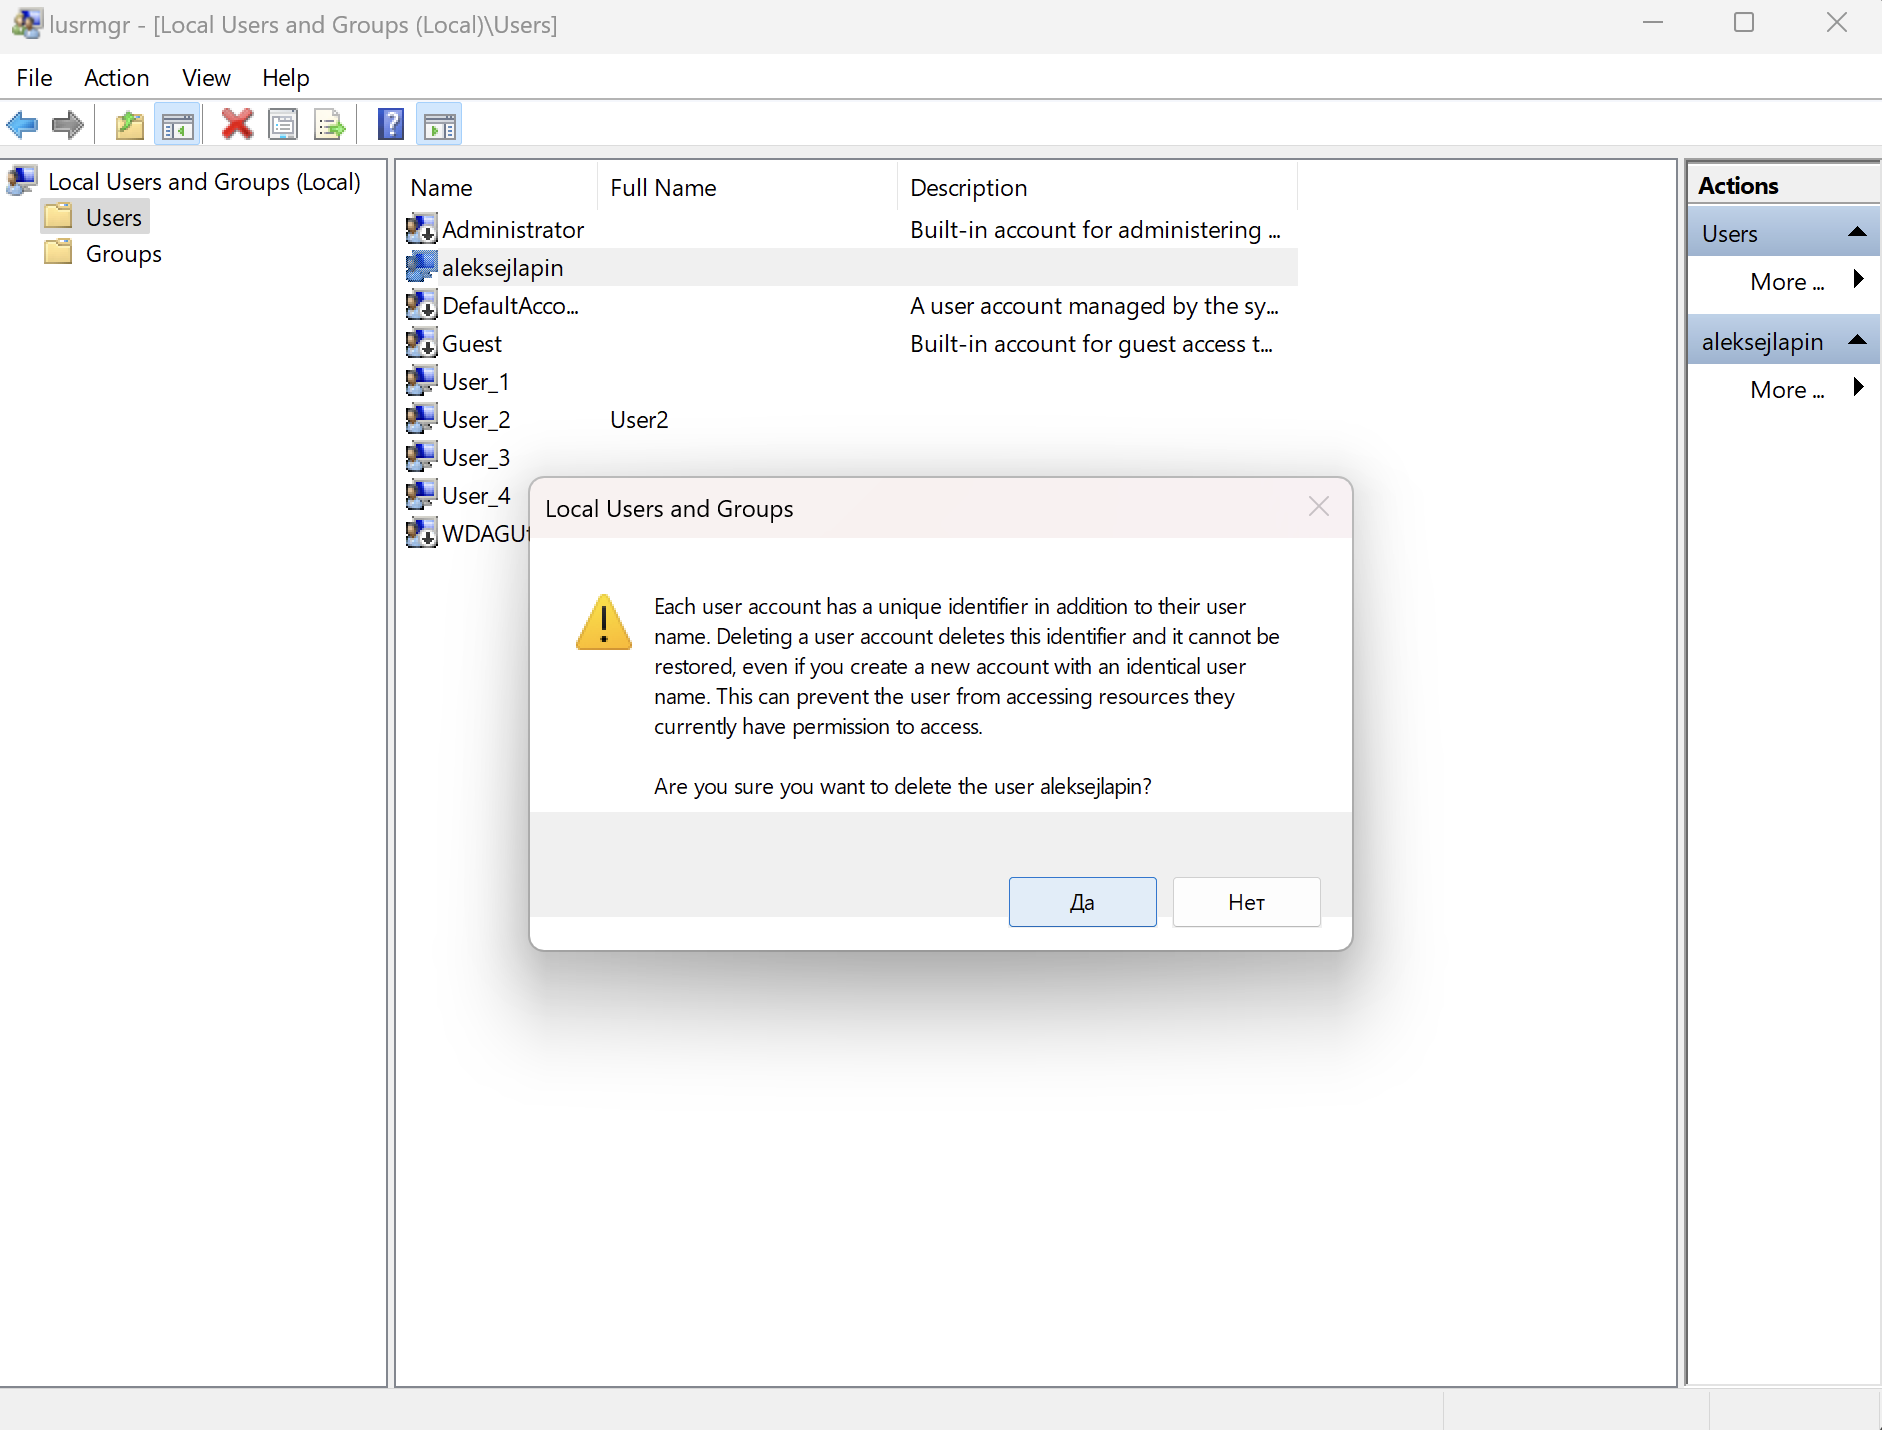
\includegraphics[width=\textwidth]{images/Screenshot 2024-12-23 at 14.51.54.png}
        \caption{}
    \end{subfigure}
    \hfill
    \begin{subfigure}[c]{0.49\textwidth}
        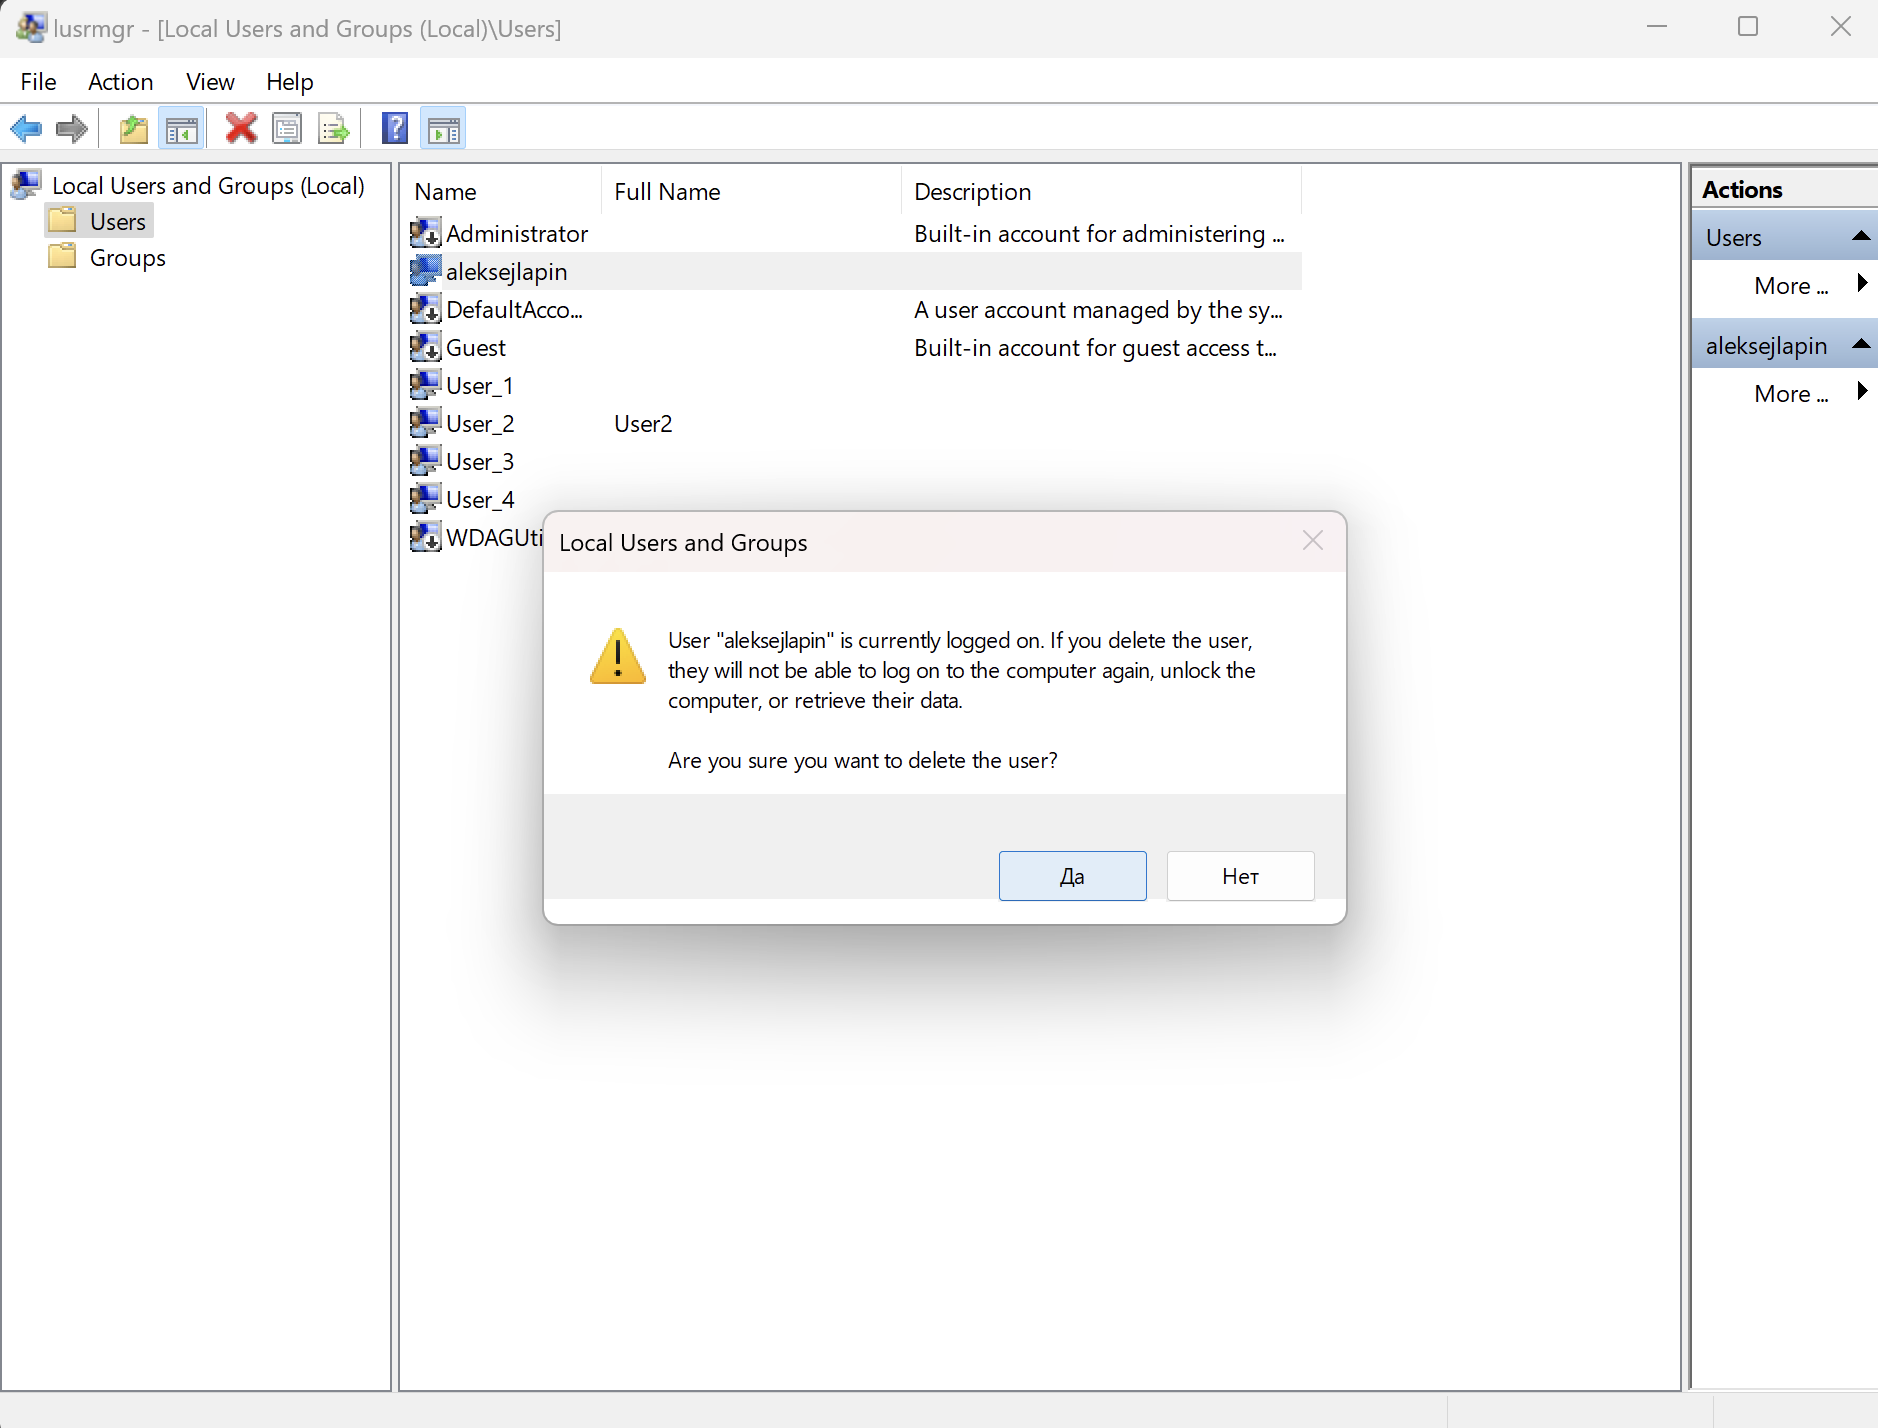
\includegraphics[width=\textwidth]{images/Screenshot 2024-12-23 at 14.52.02.png}
        \caption{}
    \end{subfigure}
    \hfill
    \begin{subfigure}[c]{0.49\textwidth}
        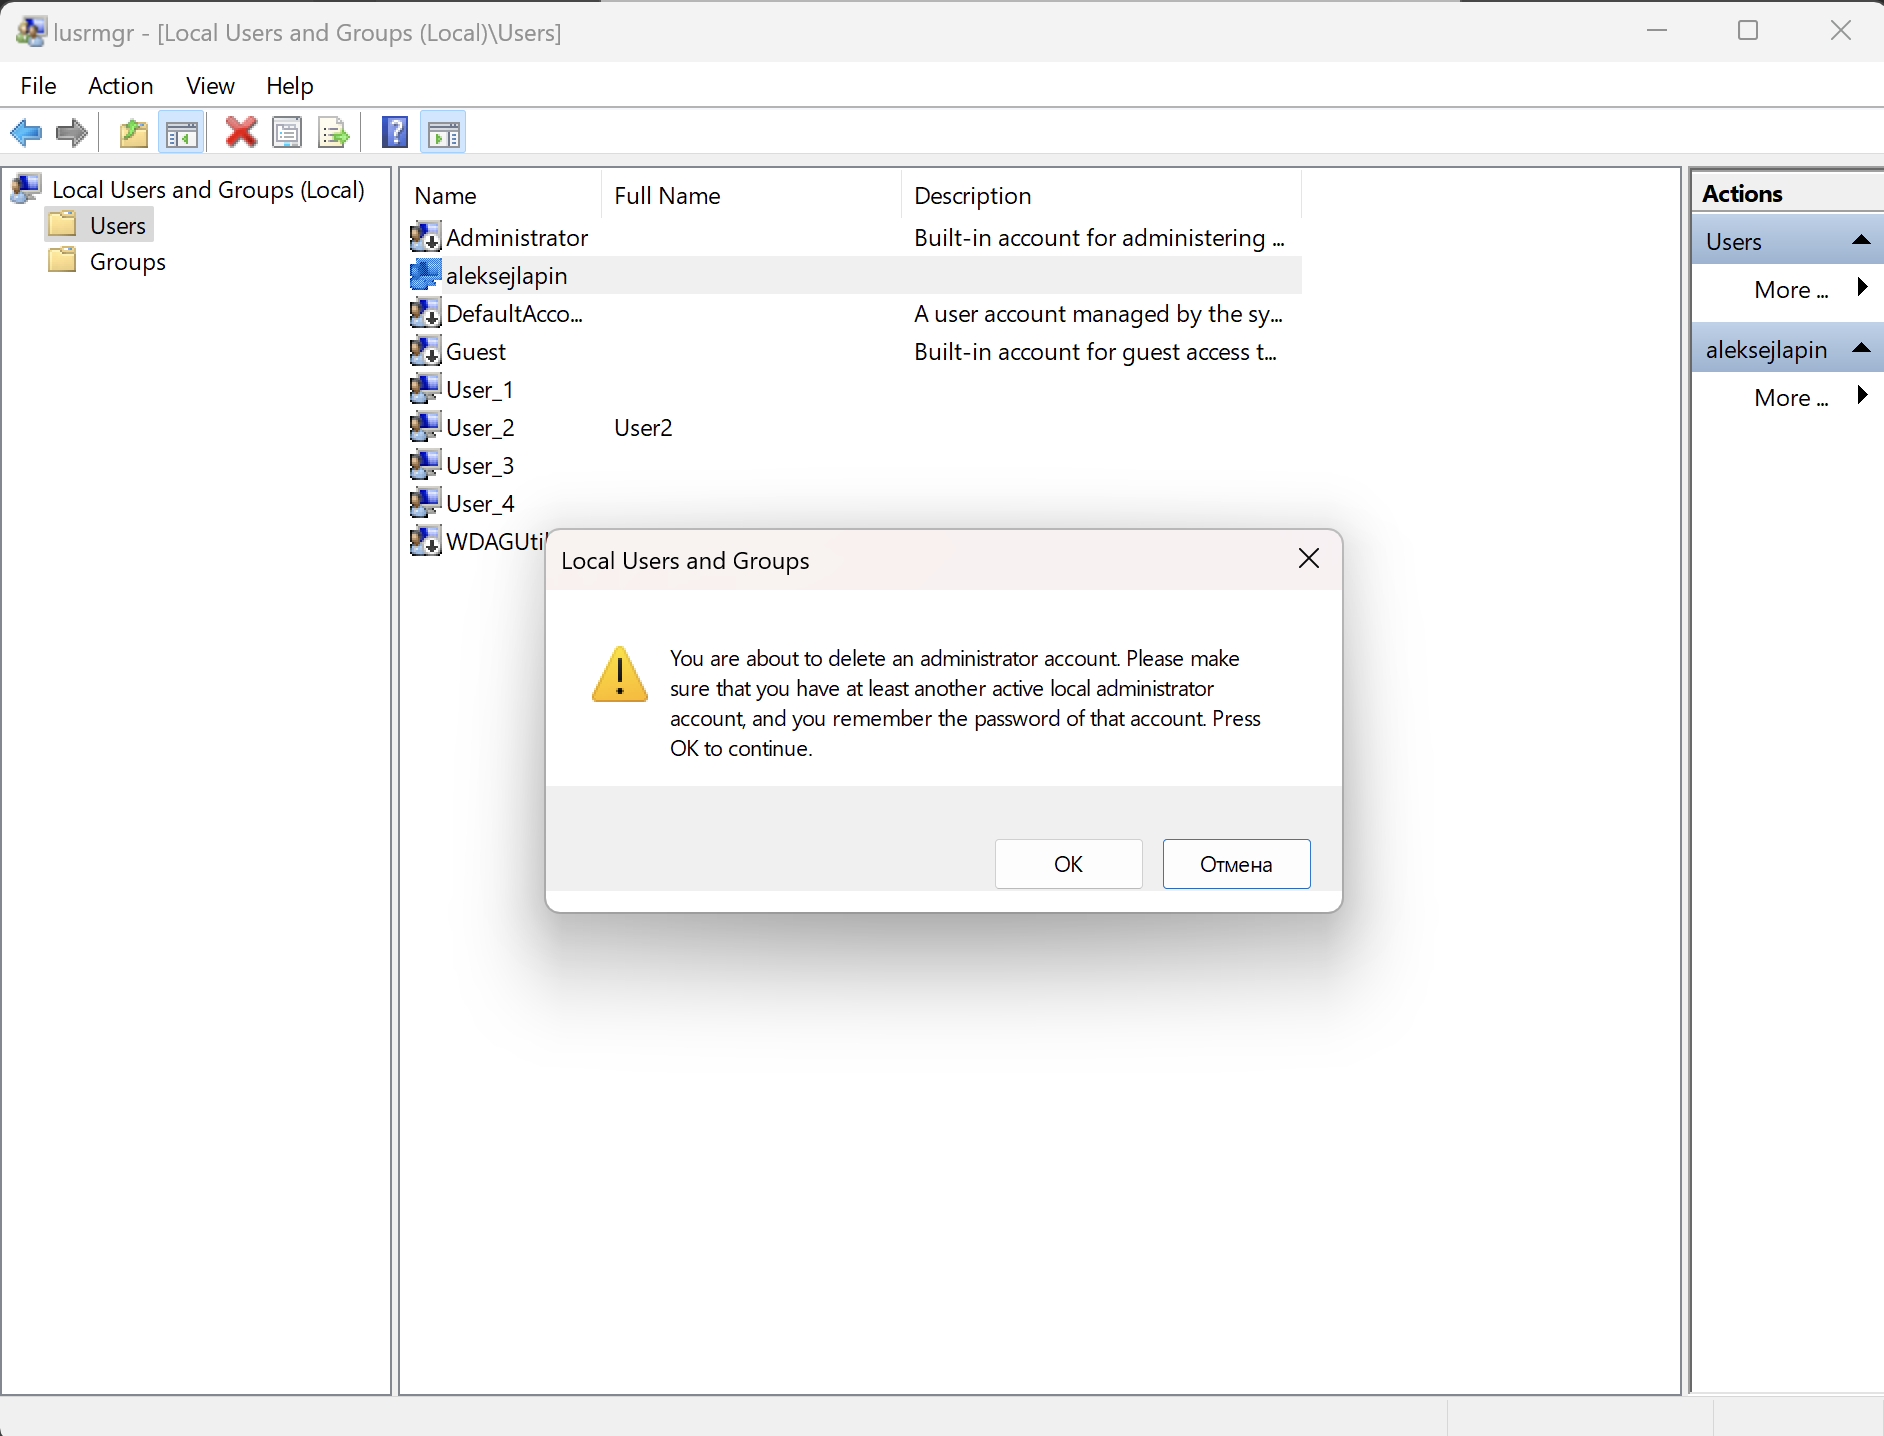
\includegraphics[width=\textwidth]{images/Screenshot 2024-12-23 at 14.52.10.png}
        \caption{}
    \end{subfigure}
    \hfill
    \begin{subfigure}[c]{0.39\textwidth}
        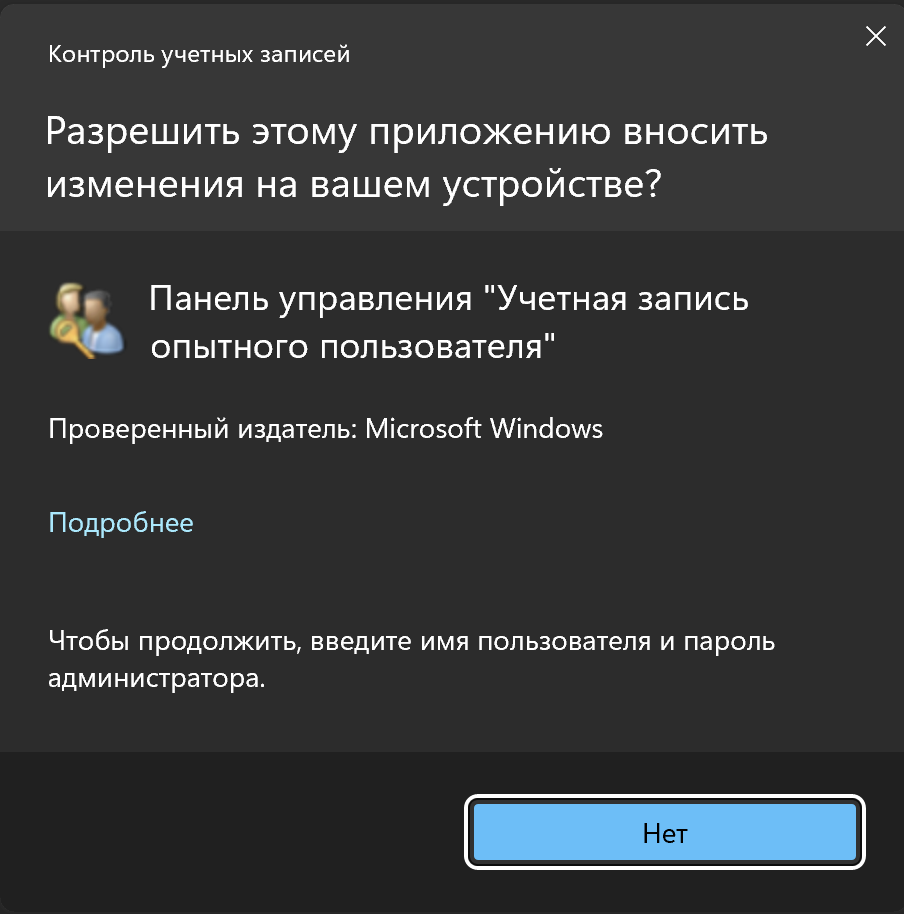
\includegraphics[width=\textwidth]{images/Screenshot 2024-12-23 at 14.52.30.png}
        \caption{}
    \end{subfigure}
    \caption{Результаты работы программы}
\end{figure}

\nchapter{Кто такие КИИ? Как понять, относитесь вы к ним или нет?}
\begin{tcolorbox}[colback=white!95!gray, colframe=teal, title=Определения]
    \textbf{Критическая информационная инфраструктура (сокращенно - КИИ)} – это информационные системы, информационно-телекоммуникационные сети, автоматизированные системы управления субъектов КИИ, а также сети электросвязи, используемые для организации их взаимодействия.\\

    \textbf{Субъекты КИИ} – это компании, работающие в стратегически важных для государства областях, таких как здравоохранение, наука, транспорт, связь, энергетика, банковская сфера, топливно-энергетический комплекс, в области атомной энергии, оборонной, ракетно-космической, горнодобывающей, металлургической и химической промышленности, а также организации, обеспечивающие взаимодействие систем или сетей КИИ.\\

    \textbf{Категория значимости объекта КИИ} может принимать одно из трех значений (где самая высокая категория - первая, самая низкая - третья) и зависит от количественных показателей значимости этого объекта в социальной, политической, экономической и оборонной сферах. Например, если компьютерный инцидент на объекте КИИ может привести к причинению ущерба жизни и здоровью более 500 граждан, то объекту присваивается максимальная первая категория, а если услуги связи в результате инцидента КИИ могут стать недоступны для 3 тыс. - 1 млн. абонентов, то объекту присваивается минимальная третья категория.
\end{tcolorbox}

В России понятие КИИ регулируется \textbf{Федеральным законом №187-ФЗ «О безопасности критической информационной инфраструктуры Российской Федерации»}, вступившим в силу 1 января 2018 года. Этот закон определяет основные принципы защиты КИИ и устанавливает ответственность за обеспечение их безопасности\cite{securityvision}.

\section{Основные элементы КИИ}
\begin{itemize}
    \item \textbf{Объекты КИИ:}
          \begin{itemize}
              \item Информационные системы.
              \item Информационно-телекоммуникационные сети.
              \item Автоматизированные системы управления.
              \item Сети электросвязи, используемые для организации взаимодействия объектов КИИ.
          \end{itemize}
    \item \textbf{Субъекты КИИ:}
          \begin{itemize}
              \item Государственные органы и учреждения.
              \item Российские юридические лица и индивидуальные предприниматели.
              \item Организации, работающие в стратегически важных сферах (здравоохранение, транспорт, связь и др.).
          \end{itemize}
\end{itemize}

\section{Категоризация и значимость КИИ}
Объекты КИИ делятся на \textbf{значимые} и \textbf{незначимые}. Значимые объекты КИИ (ЗОКИИ) классифицируются по категориям значимости от 1 до 3:

\begin{enumerate}
    \item \textbf{Категория 1:} Наивысшая значимость. Нарушение безопасности может привести к серьезным последствиям.
    \item \textbf{Категория 2:} Средняя значимость. Нарушение безопасности может вызвать значительный ущерб.
    \item \textbf{Категория 3:} Низкая значимость. Последствия ограничены и не наносят существенного ущерба.
\end{enumerate}

\section{Практическое применение КИИ: сектора и примеры}
КИИ охватывает широкий спектр секторов экономики и государственного управления. Примеры включают:

\begin{itemize}
    \item \textbf{Энергетика:} Системы управления электросетями.
    \item \textbf{Здравоохранение:} Информационные системы больниц и медицинских учреждений.
    \item \textbf{Транспорт:} Управление железными дорогами, аэропортами.
    \item \textbf{Связь:} Телекоммуникационные сети и инфраструктура.
    \item \textbf{Финансы:} Банковские информационные системы.
    \item \textbf{Оборонная промышленность:} Системы управления оборонными объектами.
\end{itemize}

\section{Как понять, относитесь ли вы к КИИ?}
Чтобы понять, относитесь ли вы к КИИ, задайте себе следующие вопросы:
\begin{enumerate}
    \item Вы работаете в одной из стратегически важных отраслей (энергетика, здравоохранение, связь и т.д.)?
    \item Ваши клиенты являются субъектами КИИ?
    \item Вам предъявляются строгие требования по информационной безопасности?
\end{enumerate}

Если ответы на большинство вопросов положительные, ваша организация, вероятно, относится к КИИ или взаимодействует с субъектами КИИ\cite{habr_kii}.


\begin{figure}[H]
    \centering
    \begin{subfigure}[c]{0.49\textwidth}
        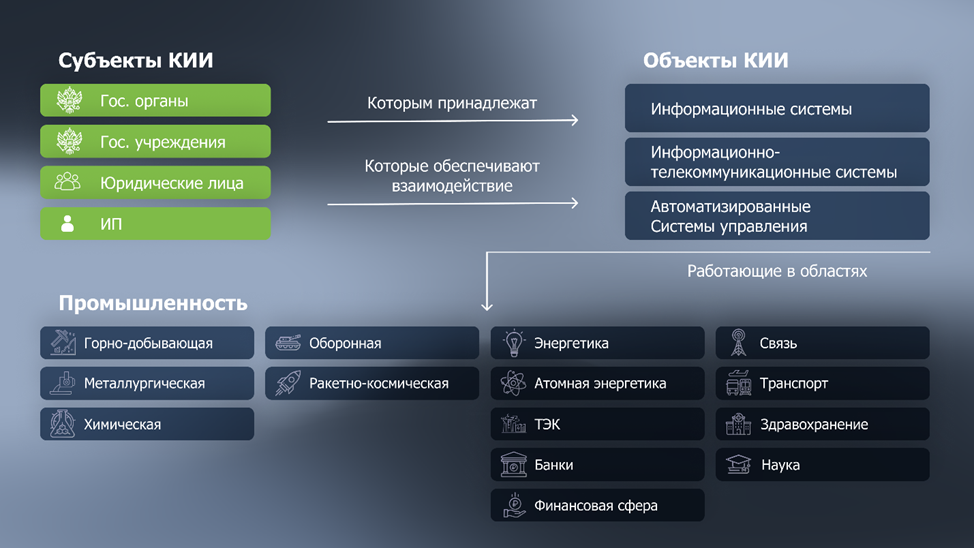
\includegraphics[width=\textwidth]{images/shema-subjects-objects.png}
        \caption{Схема субъектов и объектов КИИ}
    \end{subfigure}
    \begin{subfigure}[c]{0.49\textwidth}
        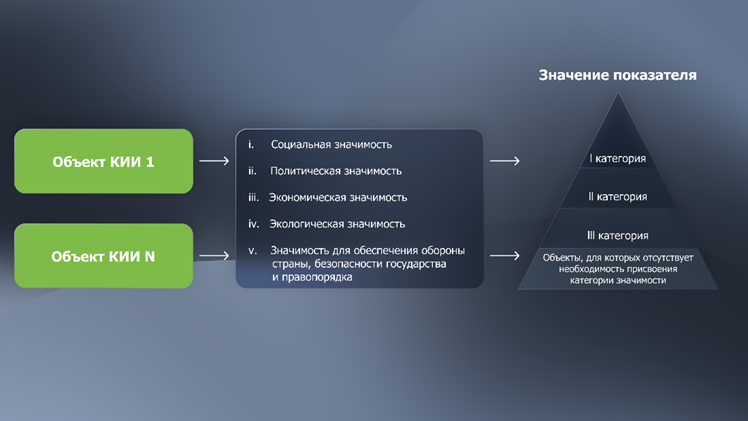
\includegraphics[width=\textwidth]{images/shema-importance-objects.png}
        \caption{Схема категорий значимости объектов КИИ}
    \end{subfigure}
    \begin{subfigure}[c]{0.49\textwidth}
        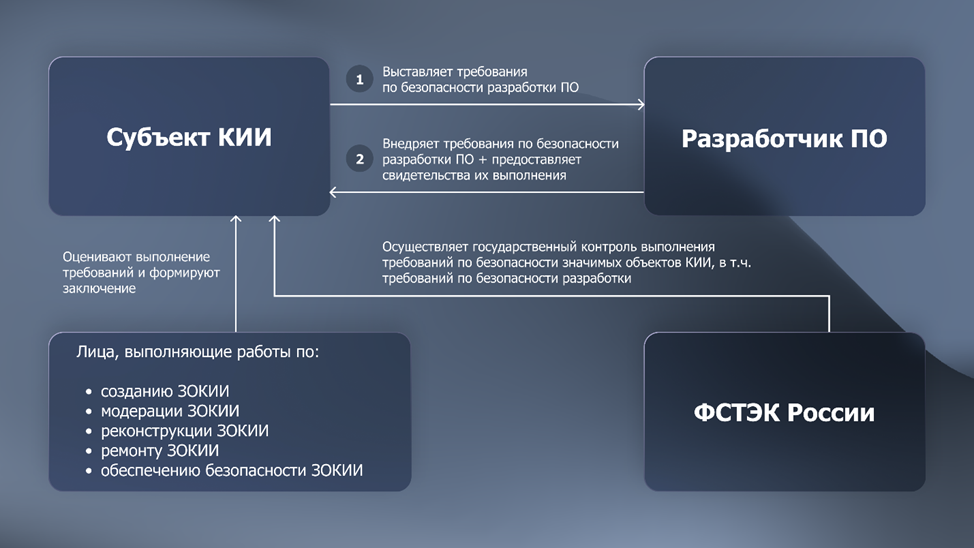
\includegraphics[width=\textwidth]{images/developer.png}
        \caption{Место компании-разработчика ПО в обеспечении безопасности КИИ}
    \end{subfigure}
\end{figure}

\printbibliography[title=Список литературы]
\end{document}
